% Options for packages loaded elsewhere
% Options for packages loaded elsewhere
\PassOptionsToPackage{unicode}{hyperref}
\PassOptionsToPackage{hyphens}{url}
\PassOptionsToPackage{dvipsnames,svgnames,x11names}{xcolor}
%
\documentclass[
  english,
  letterpaper,
  DIV=11,
  numbers=noendperiod]{scrreprt}
\usepackage{xcolor}
\usepackage{amsmath,amssymb}
\setcounter{secnumdepth}{5}
\usepackage{iftex}
\ifPDFTeX
  \usepackage[T1]{fontenc}
  \usepackage[utf8]{inputenc}
  \usepackage{textcomp} % provide euro and other symbols
\else % if luatex or xetex
  \usepackage{unicode-math} % this also loads fontspec
  \defaultfontfeatures{Scale=MatchLowercase}
  \defaultfontfeatures[\rmfamily]{Ligatures=TeX,Scale=1}
\fi
\usepackage{lmodern}
\ifPDFTeX\else
  % xetex/luatex font selection
\fi
% Use upquote if available, for straight quotes in verbatim environments
\IfFileExists{upquote.sty}{\usepackage{upquote}}{}
\IfFileExists{microtype.sty}{% use microtype if available
  \usepackage[]{microtype}
  \UseMicrotypeSet[protrusion]{basicmath} % disable protrusion for tt fonts
}{}
\makeatletter
\@ifundefined{KOMAClassName}{% if non-KOMA class
  \IfFileExists{parskip.sty}{%
    \usepackage{parskip}
  }{% else
    \setlength{\parindent}{0pt}
    \setlength{\parskip}{6pt plus 2pt minus 1pt}}
}{% if KOMA class
  \KOMAoptions{parskip=half}}
\makeatother
% Make \paragraph and \subparagraph free-standing
\makeatletter
\ifx\paragraph\undefined\else
  \let\oldparagraph\paragraph
  \renewcommand{\paragraph}{
    \@ifstar
      \xxxParagraphStar
      \xxxParagraphNoStar
  }
  \newcommand{\xxxParagraphStar}[1]{\oldparagraph*{#1}\mbox{}}
  \newcommand{\xxxParagraphNoStar}[1]{\oldparagraph{#1}\mbox{}}
\fi
\ifx\subparagraph\undefined\else
  \let\oldsubparagraph\subparagraph
  \renewcommand{\subparagraph}{
    \@ifstar
      \xxxSubParagraphStar
      \xxxSubParagraphNoStar
  }
  \newcommand{\xxxSubParagraphStar}[1]{\oldsubparagraph*{#1}\mbox{}}
  \newcommand{\xxxSubParagraphNoStar}[1]{\oldsubparagraph{#1}\mbox{}}
\fi
\makeatother

\usepackage{color}
\usepackage{fancyvrb}
\newcommand{\VerbBar}{|}
\newcommand{\VERB}{\Verb[commandchars=\\\{\}]}
\DefineVerbatimEnvironment{Highlighting}{Verbatim}{commandchars=\\\{\}}
% Add ',fontsize=\small' for more characters per line
\usepackage{framed}
\definecolor{shadecolor}{RGB}{241,243,245}
\newenvironment{Shaded}{\begin{snugshade}}{\end{snugshade}}
\newcommand{\AlertTok}[1]{\textcolor[rgb]{0.68,0.00,0.00}{#1}}
\newcommand{\AnnotationTok}[1]{\textcolor[rgb]{0.37,0.37,0.37}{#1}}
\newcommand{\AttributeTok}[1]{\textcolor[rgb]{0.40,0.45,0.13}{#1}}
\newcommand{\BaseNTok}[1]{\textcolor[rgb]{0.68,0.00,0.00}{#1}}
\newcommand{\BuiltInTok}[1]{\textcolor[rgb]{0.00,0.23,0.31}{#1}}
\newcommand{\CharTok}[1]{\textcolor[rgb]{0.13,0.47,0.30}{#1}}
\newcommand{\CommentTok}[1]{\textcolor[rgb]{0.37,0.37,0.37}{#1}}
\newcommand{\CommentVarTok}[1]{\textcolor[rgb]{0.37,0.37,0.37}{\textit{#1}}}
\newcommand{\ConstantTok}[1]{\textcolor[rgb]{0.56,0.35,0.01}{#1}}
\newcommand{\ControlFlowTok}[1]{\textcolor[rgb]{0.00,0.23,0.31}{\textbf{#1}}}
\newcommand{\DataTypeTok}[1]{\textcolor[rgb]{0.68,0.00,0.00}{#1}}
\newcommand{\DecValTok}[1]{\textcolor[rgb]{0.68,0.00,0.00}{#1}}
\newcommand{\DocumentationTok}[1]{\textcolor[rgb]{0.37,0.37,0.37}{\textit{#1}}}
\newcommand{\ErrorTok}[1]{\textcolor[rgb]{0.68,0.00,0.00}{#1}}
\newcommand{\ExtensionTok}[1]{\textcolor[rgb]{0.00,0.23,0.31}{#1}}
\newcommand{\FloatTok}[1]{\textcolor[rgb]{0.68,0.00,0.00}{#1}}
\newcommand{\FunctionTok}[1]{\textcolor[rgb]{0.28,0.35,0.67}{#1}}
\newcommand{\ImportTok}[1]{\textcolor[rgb]{0.00,0.46,0.62}{#1}}
\newcommand{\InformationTok}[1]{\textcolor[rgb]{0.37,0.37,0.37}{#1}}
\newcommand{\KeywordTok}[1]{\textcolor[rgb]{0.00,0.23,0.31}{\textbf{#1}}}
\newcommand{\NormalTok}[1]{\textcolor[rgb]{0.00,0.23,0.31}{#1}}
\newcommand{\OperatorTok}[1]{\textcolor[rgb]{0.37,0.37,0.37}{#1}}
\newcommand{\OtherTok}[1]{\textcolor[rgb]{0.00,0.23,0.31}{#1}}
\newcommand{\PreprocessorTok}[1]{\textcolor[rgb]{0.68,0.00,0.00}{#1}}
\newcommand{\RegionMarkerTok}[1]{\textcolor[rgb]{0.00,0.23,0.31}{#1}}
\newcommand{\SpecialCharTok}[1]{\textcolor[rgb]{0.37,0.37,0.37}{#1}}
\newcommand{\SpecialStringTok}[1]{\textcolor[rgb]{0.13,0.47,0.30}{#1}}
\newcommand{\StringTok}[1]{\textcolor[rgb]{0.13,0.47,0.30}{#1}}
\newcommand{\VariableTok}[1]{\textcolor[rgb]{0.07,0.07,0.07}{#1}}
\newcommand{\VerbatimStringTok}[1]{\textcolor[rgb]{0.13,0.47,0.30}{#1}}
\newcommand{\WarningTok}[1]{\textcolor[rgb]{0.37,0.37,0.37}{\textit{#1}}}

\usepackage{longtable,booktabs,array}
\usepackage{calc} % for calculating minipage widths
% Correct order of tables after \paragraph or \subparagraph
\usepackage{etoolbox}
\makeatletter
\patchcmd\longtable{\par}{\if@noskipsec\mbox{}\fi\par}{}{}
\makeatother
% Allow footnotes in longtable head/foot
\IfFileExists{footnotehyper.sty}{\usepackage{footnotehyper}}{\usepackage{footnote}}
\makesavenoteenv{longtable}
\usepackage{graphicx}
\makeatletter
\newsavebox\pandoc@box
\newcommand*\pandocbounded[1]{% scales image to fit in text height/width
  \sbox\pandoc@box{#1}%
  \Gscale@div\@tempa{\textheight}{\dimexpr\ht\pandoc@box+\dp\pandoc@box\relax}%
  \Gscale@div\@tempb{\linewidth}{\wd\pandoc@box}%
  \ifdim\@tempb\p@<\@tempa\p@\let\@tempa\@tempb\fi% select the smaller of both
  \ifdim\@tempa\p@<\p@\scalebox{\@tempa}{\usebox\pandoc@box}%
  \else\usebox{\pandoc@box}%
  \fi%
}
% Set default figure placement to htbp
\def\fps@figure{htbp}
\makeatother



\ifLuaTeX
\usepackage[bidi=basic]{babel}
\else
\usepackage[bidi=default]{babel}
\fi
% get rid of language-specific shorthands (see #6817):
\let\LanguageShortHands\languageshorthands
\def\languageshorthands#1{}
\ifLuaTeX
  \usepackage[english]{selnolig} % disable illegal ligatures
\fi


\setlength{\emergencystretch}{3em} % prevent overfull lines

\providecommand{\tightlist}{%
  \setlength{\itemsep}{0pt}\setlength{\parskip}{0pt}}



 


\KOMAoption{captions}{tableheading}
\makeatletter
\@ifpackageloaded{tcolorbox}{}{\usepackage[skins,breakable]{tcolorbox}}
\@ifpackageloaded{fontawesome5}{}{\usepackage{fontawesome5}}
\definecolor{quarto-callout-color}{HTML}{909090}
\definecolor{quarto-callout-note-color}{HTML}{0758E5}
\definecolor{quarto-callout-important-color}{HTML}{CC1914}
\definecolor{quarto-callout-warning-color}{HTML}{EB9113}
\definecolor{quarto-callout-tip-color}{HTML}{00A047}
\definecolor{quarto-callout-caution-color}{HTML}{FC5300}
\definecolor{quarto-callout-color-frame}{HTML}{acacac}
\definecolor{quarto-callout-note-color-frame}{HTML}{4582ec}
\definecolor{quarto-callout-important-color-frame}{HTML}{d9534f}
\definecolor{quarto-callout-warning-color-frame}{HTML}{f0ad4e}
\definecolor{quarto-callout-tip-color-frame}{HTML}{02b875}
\definecolor{quarto-callout-caution-color-frame}{HTML}{fd7e14}
\makeatother
\makeatletter
\@ifpackageloaded{bookmark}{}{\usepackage{bookmark}}
\makeatother
\makeatletter
\@ifpackageloaded{caption}{}{\usepackage{caption}}
\AtBeginDocument{%
\ifdefined\contentsname
  \renewcommand*\contentsname{Table of contents}
\else
  \newcommand\contentsname{Table of contents}
\fi
\ifdefined\listfigurename
  \renewcommand*\listfigurename{List of Figures}
\else
  \newcommand\listfigurename{List of Figures}
\fi
\ifdefined\listtablename
  \renewcommand*\listtablename{List of Tables}
\else
  \newcommand\listtablename{List of Tables}
\fi
\ifdefined\figurename
  \renewcommand*\figurename{Figure}
\else
  \newcommand\figurename{Figure}
\fi
\ifdefined\tablename
  \renewcommand*\tablename{Table}
\else
  \newcommand\tablename{Table}
\fi
}
\@ifpackageloaded{float}{}{\usepackage{float}}
\floatstyle{ruled}
\@ifundefined{c@chapter}{\newfloat{codelisting}{h}{lop}}{\newfloat{codelisting}{h}{lop}[chapter]}
\floatname{codelisting}{Listing}
\newcommand*\listoflistings{\listof{codelisting}{List of Listings}}
\makeatother
\makeatletter
\makeatother
\makeatletter
\@ifpackageloaded{caption}{}{\usepackage{caption}}
\@ifpackageloaded{subcaption}{}{\usepackage{subcaption}}
\makeatother
\usepackage{bookmark}
\IfFileExists{xurl.sty}{\usepackage{xurl}}{} % add URL line breaks if available
\urlstyle{same}
\hypersetup{
  pdftitle={The Quantitative Playbook for Public Health Research in R},
  pdfauthor={Shane McCarty, PhD},
  pdflang={en},
  colorlinks=true,
  linkcolor={blue},
  filecolor={Maroon},
  citecolor={Blue},
  urlcolor={Blue},
  pdfcreator={LaTeX via pandoc}}


\title{The Quantitative Playbook for Public Health Research in R}
\usepackage{etoolbox}
\makeatletter
\providecommand{\subtitle}[1]{% add subtitle to \maketitle
  \apptocmd{\@title}{\par {\large #1 \par}}{}{}
}
\makeatother
\subtitle{The R Plays to Promote and Protect Health}
\author{Shane McCarty, PhD}
\date{2025-10-14}
\begin{document}
\maketitle

\renewcommand*\contentsname{Table of contents}
{
\hypersetup{linkcolor=}
\setcounter{tocdepth}{2}
\tableofcontents
}

\bookmarksetup{startatroot}

\chapter*{Preface}\label{preface}
\addcontentsline{toc}{chapter}{Preface}

\markboth{Preface}{Preface}

The most successful sports teams rely on well-designed plays to navigate
complex game situations, the FRI Public Health research stream uses
strategic data analysis ``plays'' to tackle the multifaceted challenges
of promoting wellbeing, preventing disease, and protecting health. Our
research stream explores the intricate biopsychosocial factors affecting
human physical and mental health by collecting physiological data
through wearables like MUSE S and Fitbits, psychological insights via
survey questionnaires and interviews, and behavioral patterns through
online experiments. Like a coach calling the right play at the crucial
moment, this playbook equips you and your research teams with proven
strategies for importing, tidying, transforming, visualizing, modeling,
and communicating the mixed-methods data that helps us connect the dots
between social, political, commercial, and economic determinants of
health behavior, outcomes, and inequities. Each ``play'' in this guide
has been field-tested by research teams who have successfully used
quantitative and qualitative approaches to answer pressing questions
about physical and mental health. Whether you're facing a complex
dataset for the first time or looking to refine your analytical
strategy, this playbook offers guidance for you to turn data into
information, information into knowledge, and knowledge into wisdom in
order to improve public health outcomes.

To learn more about the FRI Public Health stream, visit us at:
\url{https://fripublichealth.quarto.pub}.

\part{Introduction}

\chapter{The Quantitative Playbook for Public Health Research in
R}\label{the-quantitative-playbook-for-public-health-research-in-r}

Students in the \href{https://fripublichealth.quarto.pub}{FRI Public
Health research stream at Binghamton University} explore a variety of
biopsychosocial factors affecting human physical and mental health. This
playbook includes a variety of ``plays'' (R code) that students in the
quantitative data analysis track can use for their team-based research
projects.

\section{The Data Analysis Workflow}\label{the-data-analysis-workflow}

This playbook follows the data science workflow in R for Data Science
(2e) (\href{https://r4ds.hadley.nz/whole-game.html}{Hadley, 2023}) to
help researchers examine the prevalence of disease and wellbeing
indicators, describe health patterns, identify associations between
(risk/protective/promotive) determinants and (positive/negative) health
outcomes, and produce a reproducible scientific report with R and
Quarto.

By the end of this guide, you will be able to:

\begin{enumerate}
\def\labelenumi{\arabic{enumi}.}
\tightlist
\item
  \textbf{Import} - Load data from various files, such as text (.csv),
  excel (.xlsx), and SPSS (.sav)
\item
  \textbf{Tidy} - Organize data into a consistent, analysis-ready
  structure
\item
  \textbf{Transform} - Clean, recode, and create new variables using
  dplyr
\item
  \textbf{Visualize} - Create informative graphs and charts with ggplot2
\item
  \textbf{Model} - Apply statistical methods (e.g., regression, paired
  t-test) to answer questions
\item
  \textbf{Communicate} - Generate reproducible reports with Quarto
\item
  \textbf{Publish --} Use transparent practices to produce multiple
  products (e.g., report, manuscript, presentation)
\end{enumerate}

Each section builds on previous concepts, taking you from raw data files
to polished, publication-ready, transparent, and reproducible scientific
report.

\subsection{What Makes This Guide
Different?}\label{what-makes-this-guide-different}

\begin{itemize}
\tightlist
\item
  \textbf{Interactive Learning}: Some code examples can be copy and
  pasted into your .R script, .qmd markdown report file, or run in the
  console. Some chapters include code examples that run directly in your
  browser using \href{https://docs.r-wasm.org/webr/latest/}{WebR}---no
  software installation required
\item
  \textbf{Real Public Health Data}: Examples use datasets on
  \href{https://www.kaggle.com/code/pralabhpoudel/does-smoking-makes-your-insurance-high}{insurance
  claims from kaggle}, oral health and diabetes (cohort 10), health
  beliefs (cohort 11), and related surveys
\item
  \textbf{Complete Workflow}: Covers every step from raw data to
  publication-ready reports
\item
  \textbf{Practical Focus}: Emphasizes ``plays'' (R code chunks) you'll
  actually use in public health research and practice
\end{itemize}

\section{Prerequisites}\label{prerequisites}

\textbf{Technical Requirements:}

\begin{itemize}
\item
  A web browser (Chrome, Firefox, Safari, or Edge) for interactive WebR
  examples
\item
  Posit Cloud in a browser or R/R Studio on your computer
\end{itemize}

\textbf{Background Knowledge:}

\begin{itemize}
\item
  Basic familiarity with public health concepts
\item
  Introductory statistics (descriptive statistics, hypothesis testing,
  p-values)
\item
  Motivation to learn more R programming (with limited R experience!)
\end{itemize}

\section{How to Cite This Guide}\label{how-to-cite-this-guide}

You can cite this guide as McCarty, S. (Ed.). (2025). \emph{The
Quantitative Playbook for Public Health Research in R}. Or, you can cite
a specific chapter: Silhavy, A. \& McCarty, S. (2025). Introduction to
ggplot2: Creating publication-ready visualizations. \emph{The
Quantitative Playbook for Public Health Research in R.}

\subsection{Authors}\label{authors}

\begin{itemize}
\item
  Editor: \href{https://shane.quarto.pub}{Shane McCarty, PhD}
\item
  Chapter Authors

  \begin{itemize}
  \item
    Allison Anemone
  \item
    Mara Estreich
  \item
    \hyperref[0]{Zihan Hei}
  \item
    Jeff John
  \item
    Gavin Rualo
  \item
    Erica Sava
  \item
    Andrew Silhavy
  \item
    Zach Spiegel
  \end{itemize}
\end{itemize}

After generating original content or sourcing from vetted R resources
(e.g., Posit, datacamp, R for Data Science), claude.ai was used to
create chapter summaries based on the chapter content and code. For some
chapters, claude.ai was used to simplify, refine, or improve existing
code chunks.

\chapter{Example Reports}\label{example-reports}

Shane McCarty \& Zihan Hei

\hfill\break

\begin{description}
\item[Replication or reproducibility crisis]
growing concern about the inability to reproduce published scientific
research findings
\end{description}

A \emph{Nature} paper by
\href{https://www.nature.com/articles/533452a}{Baker (2016)} states:
``More than 70\% of researchers have tried and failed to reproduce
another scientist's experiments, and more than half have failed to
reproduce their own experiments.''

The failure to reproduce research is a function of systems pressure
(defunding of public higher education), \emph{intentional actions}
(fraudulent scientific practices), \emph{unintentional}
\emph{decision-making} (e.g., human error when clicking software, poor
note-taking), and \emph{scientific} \emph{training} (e.g., methodology
sections without clear protocols and details). Reproducible research is
both an intentional practice and the outcome of scientific training
emphasizing a specific workflow.

A primary objective of this playbook is to increase the reproducibility
of public health research using line-by-line coding in R with Quarto for
publishing the research with code chunks to confirm accuracy.

\chapter{Reproducible Reports}\label{reproducible-reports}

You and your team will produce a reproducible Quarto Markdown report
(\texttt{.qmd}) for your individual report and team manuscript. Specific
instructions are provided in the next chapter.

Quarto provided two examples of a reproducible report and manuscript:

\begin{itemize}
\item
  \href{https://quarto-dev.github.io/quarto-gallery/page-layout/tufte.html}{Standard
  Quarto Report Example}
\item
  \href{https://quarto-ext.github.io/manuscript-template-jupyter/}{Standard
  Quarto Manuscript Example}
\end{itemize}

The FRI Public Health Lab has produced Quarto manuscripts from active
research projects:

\begin{itemize}
\item
  \href{https://zihanhei.quarto.pub/avoider-report/}{Health Avoiders
  Report}
\item
  \href{https://fripublichealth.quarto.pub/zerosum/}{Zero Sum Full
  Report}
\item
  \href{https://fripublichealth.quarto.pub/zerosum/example-preview.html}{Zero
  Sum Mini Report}
\end{itemize}

\chapter{Start Quarto Markdown
Document}\label{start-quarto-markdown-document}

Create .qmd, Write in Markdown, Add Meta-data in YAML, and Create Code
Chunks

This chapter introduces students to creating and structuring Quarto
markdown documents (.qmd) for reproducible research. Students learn to
set up new Quarto documents, configure metadata using YAML headers, and
write formatted text using markdown syntax. The chapter demonstrates
proper code chunk structure with descriptive labels, detailed figure
captions, and execution options. Students explore essential practices
including file naming conventions, environment management, and
documentation through code sources and explanations. By the end of this
chapter, students will understand how to create professional,
well-documented Quarto reports that integrate narrative text with
embedded R code, following reproducible research standards for public
health manuscripts.

\hfill\break

\begin{tcolorbox}[enhanced jigsaw, title=\textcolor{quarto-callout-tip-color}{\faLightbulb}\hspace{0.5em}{📖 Learning Resources}, opacityback=0, colframe=quarto-callout-tip-color-frame, rightrule=.15mm, left=2mm, toprule=.15mm, leftrule=.75mm, titlerule=0mm, bottomtitle=1mm, breakable, arc=.35mm, toptitle=1mm, bottomrule=.15mm, coltitle=black, opacitybacktitle=0.6, colback=white, colbacktitle=quarto-callout-tip-color!10!white]

\begin{itemize}
\tightlist
\item
  \textbf{R for Data Science}:
  \href{https://r4ds.hadley.nz/quarto.html}{Quarto}
\item
  \textbf{Website}: \href{https://quarto.org}{Quarto}
\item
  \textbf{Youtube}:

  \begin{itemize}
  \tightlist
  \item
    \href{https://www.youtube.com/watch?v=_f3latmOhew}{Getting Started
    with Quarto}
  \item
    \href{https://www.youtube.com/watch?v=EbAAmrB0luA}{Quarto for
    Academics}
  \end{itemize}
\item
  \textbf{Cheat Sheet}:
  \href{https://rstudio.github.io/cheatsheets/quarto.pdf}{Quarto}
\item
  \textbf{Posit Interactive Page}:
  \href{https://rstudio.github.io/cheatsheets/html/quarto.html}{Quarto}
\end{itemize}

\end{tcolorbox}

In your Posit Cloud window browser, you should see the \emph{source} and
\emph{visual} editor options in the top left corner of your screen. You
can toggle back and forth between the two options.

\begin{itemize}
\item
  The source option is your best option for coding in R with line items.
\item
  The visual editor is your best place to see the quarto markdown
  document (.qmd) before it is officially rendered as an HTML output.
\end{itemize}

\chapter{Create a Markdown Document}\label{create-a-markdown-document}

\begin{itemize}
\tightlist
\item
  File \textgreater{} New File \textgreater{} Quarto Document
\item
  Complete Title and Author Name, Create
\item
  File \textgreater{} Save As \textgreater{} name-it-now.qmd
\item
  Check the file shows up in your files in the bottom right window as
  .qmd file
\end{itemize}

\section{Quarto Document File Names}\label{quarto-document-file-names}

For individual lab and report quarto reports:

\begin{itemize}
\tightlist
\item
  Your individual lab was renamed to \texttt{lab.qmd}
\item
  Your results and discussion report should be named:
  \texttt{RDreport.qmd}
\item
  After submitting your \texttt{RDreport.qmd}, you should go to the
  files tab, check the box next to \texttt{RDreport.qmd} and then click
  the gear icon (More) \textgreater{} Copy \textgreater{} name it
  \texttt{name\_report.qmd}
\item
  Your final report should be named: \texttt{name\_report.qmd}
\end{itemize}

\begin{tcolorbox}[enhanced jigsaw, title=\textcolor{quarto-callout-important-color}{\faExclamation}\hspace{0.5em}{Requirement}, opacityback=0, colframe=quarto-callout-important-color-frame, rightrule=.15mm, left=2mm, toprule=.15mm, leftrule=.75mm, titlerule=0mm, bottomtitle=1mm, breakable, arc=.35mm, toptitle=1mm, bottomrule=.15mm, coltitle=black, opacitybacktitle=0.6, colback=white, colbacktitle=quarto-callout-important-color!10!white]

You must name your quarto markdown files (\texttt{.qmd}) correctly.

\end{tcolorbox}

\section{Clearing Environment in Posit
Cloud}\label{clearing-environment-in-posit-cloud}

Your previously created objects (e.g., \texttt{alldata},
\texttt{select\_data}, \texttt{VARIABLE1}) are stored in your
environment even when you return to your posit cloud account. It is
important to clear all objects from your environment before beginning
your next assignment. Also, this code is important to use when you want
to double check that your \texttt{.qmd} document will render correctly.
You can clear all of the objects and then run your entire .qmd document
to check for errors.

\begin{Shaded}
\begin{Highlighting}[]
\CommentTok{\# Remove all objects from the global environment}
\FunctionTok{rm}\NormalTok{(}\AttributeTok{list =} \FunctionTok{ls}\NormalTok{())}
\end{Highlighting}
\end{Shaded}

For your draft and final team MMR manuscript, you should: - pick one
quantitative team member to store the team files in their posit cloud
project - rename this specific posit cloud project from \#1: Vivian
-\textgreater{} \#1: Vivian \& Team (to notify me where to look for your
team's MMR work) - create a \texttt{team\_RD.qmd} file - create a
\texttt{team\_final.qmd} file

\chapter{YAML}\label{yaml}

YAML (human-readable data serialization language) has a simple syntax,
which is a structured way to organize information (aka metadata), such
as title, author, date, and format output (HTML vs.~PDF).

\begin{tcolorbox}[enhanced jigsaw, title=\textcolor{quarto-callout-important-color}{\faExclamation}\hspace{0.5em}{Requirement}, opacityback=0, colframe=quarto-callout-important-color-frame, rightrule=.15mm, left=2mm, toprule=.15mm, leftrule=.75mm, titlerule=0mm, bottomtitle=1mm, breakable, arc=.35mm, toptitle=1mm, bottomrule=.15mm, coltitle=black, opacitybacktitle=0.6, colback=white, colbacktitle=quarto-callout-important-color!10!white]

Use this YAML format at the top of ALL Quarto markdown document files
(\texttt{.qmd}).

\end{tcolorbox}

\begin{Shaded}
\begin{Highlighting}[]
\PreprocessorTok{{-}{-}{-}}

\FunctionTok{title}\KeywordTok{:}\AttributeTok{ }\StringTok{"name your final report here"}
\FunctionTok{author}\KeywordTok{:}\AttributeTok{ }\StringTok{"put your full name here"}
\FunctionTok{date}\KeywordTok{:}\AttributeTok{ }\StringTok{"3/22/2023"}
\FunctionTok{abstract}\KeywordTok{: }\CharTok{|}
\NormalTok{    TBD goes here}
\FunctionTok{format}\KeywordTok{:}\AttributeTok{ }
\AttributeTok{  }\FunctionTok{html}\KeywordTok{:}
\AttributeTok{    }\FunctionTok{fig{-}width}\KeywordTok{:}\AttributeTok{ }\DecValTok{8}
\AttributeTok{    }\FunctionTok{fig{-}height}\KeywordTok{:}\AttributeTok{ }\DecValTok{4}
\AttributeTok{    }\FunctionTok{code{-}fold}\KeywordTok{:}\AttributeTok{ }\CharTok{true}
\AttributeTok{    }
\PreprocessorTok{{-}{-}{-}}
\end{Highlighting}
\end{Shaded}

For more information, see
\href{https://quarto.org/docs/reference/formats/html.html}{YAML}.

\chapter{Markdown}\label{markdown}

You will write in the English language with
\href{https://quarto.org/docs/authoring/markdown-basics.html}{markdown}
language to format your quarto report.

\begin{Shaded}
\begin{Highlighting}[]
\NormalTok{This is a language called markdown. It is very simple. You can use}
\NormalTok{*italics*, **bold**, ***bold italics*** to produce:}
\end{Highlighting}
\end{Shaded}

\begin{itemize}
\tightlist
\item
  \emph{italics}
\item
  \textbf{bold}
\item
  \textbf{\emph{bold italics}}
\end{itemize}

\section{Verbatim Code}\label{verbatim-code}

You can use a backtick to denote code or the name of a variable by
placing a word within ``. For example, if I put EFFICACY between `` then
it returns \texttt{EFFICACY} . This will be important for naming
variables in your report.

\begin{tcolorbox}[enhanced jigsaw, title=\textcolor{quarto-callout-important-color}{\faExclamation}\hspace{0.5em}{Requirement}, opacityback=0, colframe=quarto-callout-important-color-frame, rightrule=.15mm, left=2mm, toprule=.15mm, leftrule=.75mm, titlerule=0mm, bottomtitle=1mm, breakable, arc=.35mm, toptitle=1mm, bottomrule=.15mm, coltitle=black, opacitybacktitle=0.6, colback=white, colbacktitle=quarto-callout-important-color!10!white]

Use ` ` between CAPITALIZED variable names in your report if you are
referring to the measured variable. The use of backticks is NOT
appropriate in your introduction and discussion sections, but backticks
should be used in your methods and results sections.

\end{tcolorbox}

\chapter{Code Chunks}\label{code-chunks}

A traditional R script (\texttt{.R}) involves code throughout the entire
script. A Quarto Markdown Document (\texttt{.qmd}) integrates the R
programming language with markdown language into a single document that
can include a mix of code and written content. We use
\texttt{report.qmd} and other \texttt{.qmd} files to write a
reproducible manuscript using written text within embedded code chunks.

\section{Example Code Chunk}\label{example-code-chunk}

Below is an example from the @ggplot2.qmd chapter of an informative
\texttt{label} for your code chunk and a very detailed figure caption (
\texttt{fig-cap}). Also, notice that all code chunk options start with
\texttt{\#\textbar{}} and use a \texttt{:}.

For more examples, see @ggplot2.qmd.

\begin{Shaded}
\begin{Highlighting}[]
\InformationTok{\textasciigrave{}\textasciigrave{}\textasciigrave{}\{r\}}
\CommentTok{\#| label: scatterplot{-}BMI{-}insurance}
\CommentTok{\#| fig{-}cap: A scatterplot depicting the relationship between body mass index and insurance charges with a line of best fit to demonstrate the liner relationship between the two variables}
\CommentTok{\#| eval: false}
\FunctionTok{ggplot}\NormalTok{(}\AttributeTok{data =}\NormalTok{ insurance, }\AttributeTok{mapping =} \FunctionTok{aes}\NormalTok{(}\AttributeTok{x =}\NormalTok{ bmi, }\AttributeTok{y =}\NormalTok{ charges)) }\SpecialCharTok{+}
  \FunctionTok{geom\_point}\NormalTok{() }\SpecialCharTok{+}
  \FunctionTok{geom\_smooth}\NormalTok{(}\AttributeTok{method =} \StringTok{"lm"}\NormalTok{)}

\CommentTok{\#source: Introduction to ggplot2 (Silhavy \& McCarty, 2025)}
\CommentTok{\#explanation: the insurance data is being used with BMI for the x variable and insurance charges for the year variable. geom\_point is used for scatterplots. geom\_smooth with lm adds a linear model on top of the datapoint to show the association between BMI and insurance charges}
\InformationTok{\textasciigrave{}\textasciigrave{}\textasciigrave{}}
\end{Highlighting}
\end{Shaded}

\section{Template Code Chunk}\label{template-code-chunk}

\subsection{Label for All Code Chunks}\label{label-for-all-code-chunks}

\begin{tcolorbox}[enhanced jigsaw, title=\textcolor{quarto-callout-important-color}{\faExclamation}\hspace{0.5em}{Requirement}, opacityback=0, colframe=quarto-callout-important-color-frame, rightrule=.15mm, left=2mm, toprule=.15mm, leftrule=.75mm, titlerule=0mm, bottomtitle=1mm, breakable, arc=.35mm, toptitle=1mm, bottomrule=.15mm, coltitle=black, opacitybacktitle=0.6, colback=white, colbacktitle=quarto-callout-important-color!10!white]

Every code chunk must have a \texttt{\#\textbar{}\ label:} at the start
of the chunk.

\end{tcolorbox}

\begin{Shaded}
\begin{Highlighting}[]
\InformationTok{\textasciigrave{}\textasciigrave{}\textasciigrave{}\{r\}}
\CommentTok{\#| label: this is a label that you will revise}

\InformationTok{\textasciigrave{}\textasciigrave{}\textasciigrave{}}
\end{Highlighting}
\end{Shaded}

Your \texttt{\#\textbar{}\ label:} should be lowercase with dashs
between words to create a complete object with no spaces, such as
import-data-csv or import-data-xlsx.

\begin{Shaded}
\begin{Highlighting}[]
\InformationTok{\textasciigrave{}\textasciigrave{}\textasciigrave{}\{r\}}
\CommentTok{\#| label: import{-}data{-}xlsx}

\InformationTok{\textasciigrave{}\textasciigrave{}\textasciigrave{}}
\end{Highlighting}
\end{Shaded}

\subsection{Figure Caption (Fig-Cap) for Plot Code
Chunks}\label{figure-caption-fig-cap-for-plot-code-chunks}

\begin{tcolorbox}[enhanced jigsaw, title=\textcolor{quarto-callout-important-color}{\faExclamation}\hspace{0.5em}{Requirement}, opacityback=0, colframe=quarto-callout-important-color-frame, rightrule=.15mm, left=2mm, toprule=.15mm, leftrule=.75mm, titlerule=0mm, bottomtitle=1mm, breakable, arc=.35mm, toptitle=1mm, bottomrule=.15mm, coltitle=black, opacitybacktitle=0.6, colback=white, colbacktitle=quarto-callout-important-color!10!white]

Every plot should include a detailed figure caption using
\texttt{\#\textbar{}\ fig-cap:}

\end{tcolorbox}

\begin{Shaded}
\begin{Highlighting}[]
\InformationTok{\textasciigrave{}\textasciigrave{}\textasciigrave{}\{r\}}
\CommentTok{\#| label: you{-}need{-}to{-}revise{-}this}
\CommentTok{\#| fig{-}cap: you need to revise this with detailed figure caption}

\InformationTok{\textasciigrave{}\textasciigrave{}\textasciigrave{}}
\end{Highlighting}
\end{Shaded}

\subsection{Provide Sources for ALL Code
Chunks}\label{provide-sources-for-all-code-chunks}

\begin{tcolorbox}[enhanced jigsaw, title=\textcolor{quarto-callout-important-color}{\faExclamation}\hspace{0.5em}{Requirement}, opacityback=0, colframe=quarto-callout-important-color-frame, rightrule=.15mm, left=2mm, toprule=.15mm, leftrule=.75mm, titlerule=0mm, bottomtitle=1mm, breakable, arc=.35mm, toptitle=1mm, bottomrule=.15mm, coltitle=black, opacitybacktitle=0.6, colback=white, colbacktitle=quarto-callout-important-color!10!white]

At the end of every code chunk, include the source of the code chunk so
that others can replicate your work. You should use a pseudo APA
citation format with (author, year) and website link (if possible).

\end{tcolorbox}

\begin{Shaded}
\begin{Highlighting}[]
\InformationTok{\textasciigrave{}\textasciigrave{}\textasciigrave{}\{r\}}
\CommentTok{\#| label: you{-}need{-}to{-}revise{-}this}
\CommentTok{\#| fig{-}cap: you need to revise this with detailed figure caption}

\CommentTok{\#source example 1: The FRI Playbook (McCarty, 2025)   }
\CommentTok{\#source example 2: Write Functions (Hei, 2025)   }
\CommentTok{\#source example 3: Quarto guide markdown basics: https://quarto.org/docs/authoring/markdown{-}basics.html}

\InformationTok{\textasciigrave{}\textasciigrave{}\textasciigrave{}}
\end{Highlighting}
\end{Shaded}

Notice that the format is different. The \texttt{\#source:} NOT be in
the prior \texttt{\#\textbar{}} format you used for the code chunks at
the topic. The \#source will be at the bottom of your code chunk.

\subsection{Provide Explanation for ALL Code
Chunks}\label{provide-explanation-for-all-code-chunks}

\begin{tcolorbox}[enhanced jigsaw, title=\textcolor{quarto-callout-important-color}{\faExclamation}\hspace{0.5em}{Requirement}, opacityback=0, colframe=quarto-callout-important-color-frame, rightrule=.15mm, left=2mm, toprule=.15mm, leftrule=.75mm, titlerule=0mm, bottomtitle=1mm, breakable, arc=.35mm, toptitle=1mm, bottomrule=.15mm, coltitle=black, opacitybacktitle=0.6, colback=white, colbacktitle=quarto-callout-important-color!10!white]

You will explain the code chunk in your own words using
\texttt{\#explanation:} at the bottom of your code chunk.

\end{tcolorbox}

\begin{Shaded}
\begin{Highlighting}[]
\InformationTok{\textasciigrave{}\textasciigrave{}\textasciigrave{}\{r\}}
\CommentTok{\#| label: scatterplot{-}BMI{-}insurance}
\CommentTok{\#| fig{-}cap: A scatterplot depicting the relationship between body mass index and insurance charges with a line of best fit to demonstrate the liner relationship between the two variables}
\CommentTok{\#| eval: false}

\FunctionTok{ggplot}\NormalTok{(}\AttributeTok{data =}\NormalTok{ insurance, }\AttributeTok{mapping =} \FunctionTok{aes}\NormalTok{(}\AttributeTok{x =}\NormalTok{ bmi, }\AttributeTok{y =}\NormalTok{ charges)) }\SpecialCharTok{+}
  \FunctionTok{geom\_point}\NormalTok{() }\SpecialCharTok{+}
  \FunctionTok{geom\_smooth}\NormalTok{(}\AttributeTok{method =} \StringTok{"lm"}\NormalTok{)}

\CommentTok{\#source: Introduction to ggplot2 (Silhavy \& McCarty, 2025)}
\CommentTok{\#explanation: the insurance data is being used with BMI for the x variable and insurance charges for the year variable. geom\_point is used for scatterplots. geom\_smooth with lm adds a linear model on top of the datapoint to show the association between BMI and insurance charges}
\InformationTok{\textasciigrave{}\textasciigrave{}\textasciigrave{}}
\end{Highlighting}
\end{Shaded}

\subsection{Code Chunk Options}\label{code-chunk-options}

For more information on code chunks, see
\href{https://r4ds.hadley.nz/quarto.html\#chunk-options}{code chunk
options}.

\begin{Shaded}
\begin{Highlighting}[]
\InformationTok{\textasciigrave{}\textasciigrave{}\textasciigrave{}\{r\}}
\CommentTok{\#| label: example{-}with{-}options}
\CommentTok{\#| eval: true          \# Whether to execute the code}
\CommentTok{\#| echo: fenced        \# for teaching {-}{-} this shows the code chunk options to you}
\CommentTok{\#| output: true        \# Whether to display output}
\CommentTok{\#| warning: false      \# Hide warnings}
\CommentTok{\#| message: false      \# Hide messages}
\CommentTok{\#| error: false        \# Hide errors}
\CommentTok{\#| fig{-}cap: "Caption"  \# Figure caption}
\CommentTok{\#| fig{-}width: 8        \# Figure width in inches}
\CommentTok{\#| fig{-}height: 6       \# Figure height in inches}

\CommentTok{\# Your code here below these code chunk options}
\InformationTok{\textasciigrave{}\textasciigrave{}\textasciigrave{}}
\end{Highlighting}
\end{Shaded}

\part{Importing Data}

\chapter{Exporting Survey Data}\label{exporting-survey-data}

This chapter introduces students to import qualtrics features, such as
recoding variables in qualtrics before exporting the dataset.

\hfill\break

\chapter{Exporting Survey Data}\label{exporting-survey-data-1}

\begin{itemize}
\item[$\square$]
  Log into Qualtrics: \url{https://binghamton.co1.qualtrics.com}

  \begin{itemize}
  \tightlist
  \item[$\square$]
    Under Active surveys, click on your survey
  \end{itemize}
\item[$\square$]
  Recode variables in Qualtrics

  \begin{itemize}
  \item[$\square$]
    Visit the ``Exporting Survey Data'' section in the
    \href{https://docs.google.com/presentation/d/1VGnFFuaKgtEzWRYaI04DAT4ebn_Qfxl370Nxmg2KEdc/edit?slide=id.g38c5b5e4629_0_7\#slide=id.g38c5b5e4629_0_7}{presentation
    slides}
  \item[$\square$]
    Visit ``Recode Values'' section of the
    \href{https://www.qualtrics.com/support/survey-platform/survey-module/question-options/recode-values/}{Qualtrics
    guide}
  \item[$\square$]
    Follow the instructions:
    \url{https://docs.google.com/document/d/15ynxeoIaLhABAAeDLJYV1MwQRwpI8LM24Zd3tOwxcFQ/edit?tab=t.0\#heading=h.25d8wyh38wre}
  \end{itemize}
\end{itemize}

\chapter{Exporting Survey Data}\label{exporting-survey-data-2}

\begin{itemize}
\tightlist
\item[$\square$]
  Log into Qualtrics: \url{https://binghamton.co1.qualtrics.com}

  \begin{itemize}
  \tightlist
  \item[$\square$]
    Under Active surveys, click on your survey
  \end{itemize}
\item[$\square$]
  At the top, go to Data \& Analysis tab (top navigation bar)

  \begin{itemize}
  \tightlist
  \item[$\square$]
    Ensure that ``Data'' is selected (from the second navigvation bar)
  \end{itemize}
\end{itemize}

\begin{figure}[H]

{\centering \pandocbounded{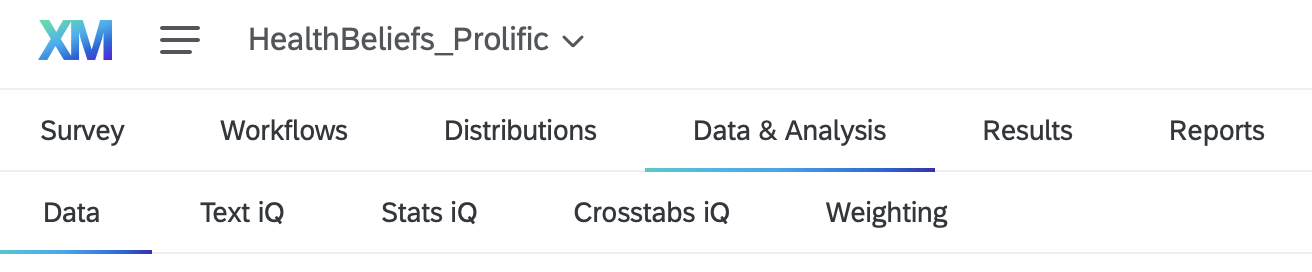
\includegraphics[keepaspectratio]{images/export-navbar.png}}

}

\caption{\emph{Click on Data \& Analysis and ensure Data is underlined
in the navigation bars.}}

\end{figure}%

\begin{itemize}
\item[$\square$]
  On the upper right side, click Export \& Import \^{}, then select
  Export Data\ldots{}
\item[$\square$]
  Download the dataset (with download all fields checked and export
  \emph{values} check -- do not select export \emph{labels} in two file
  formats:

  \begin{itemize}
  \item[$\square$]
    CSV
  \item[$\square$]
    Excel
  \end{itemize}
\item[$\square$]
  Upload both files to ``Survey Data'' folder in your Team ELN
\item[$\square$]
  Rename both files using the date MONTH.DAY.YEAR.filename.filetype
  (e.g., \texttt{03.15.2025.ProlificHealthBeliefs.csv} and
  \texttt{03.15.2025.ProlificHealthBeliefs.xlsx}).
\end{itemize}

\chapter{Importing Data Simply}\label{importing-data-simply}

TBD

\hfill\break

\section{Purpose}\label{purpose}

Importing data is the first step in the workflow.

\begin{Shaded}
\begin{Highlighting}[]
\FunctionTok{install.packages}\NormalTok{(}\StringTok{"NHANES"}\NormalTok{)}
\FunctionTok{install.packages}\NormalTok{(}\StringTok{"devtools"}\NormalTok{)}
\end{Highlighting}
\end{Shaded}

\section{First Setup the library:}\label{first-setup-the-library}

\begin{Shaded}
\begin{Highlighting}[]
\FunctionTok{library}\NormalTok{(tidyverse)}
\FunctionTok{library}\NormalTok{(psych)}
\FunctionTok{library}\NormalTok{(knitr)}
\FunctionTok{library}\NormalTok{(tibble)}
\FunctionTok{library}\NormalTok{(dplyr)}
\FunctionTok{library}\NormalTok{(tidyr)}
\FunctionTok{library}\NormalTok{(scales)     }\CommentTok{\# for number formatting like comma()}
\FunctionTok{library}\NormalTok{(english)    }\CommentTok{\# to convert numbers to words}
\FunctionTok{library}\NormalTok{(stringr)    }\CommentTok{\# for text functions like str\_c()}
\FunctionTok{library}\NormalTok{(NHANES)}
\end{Highlighting}
\end{Shaded}

\chapter{Datasets}\label{datasets}

You will learn how to import different datasets:

\begin{itemize}
\item
  datasets in R packages \texttt{NHANES} and \texttt{YRBS}
\item
  class dataset ``health beliefs (cohort 11) collected in the Research
  Methods I (ANTH206) course
\item
  team dataset ``oralhealth''
\end{itemize}

\section{File Formats}\label{file-formats}

\begin{itemize}
\item
  National Health and Nutrition Examination Survey dataset from the
  Centers for Disease Control and Prevention (CDC) using the R package
  \texttt{NHANES}
\item
  a \texttt{.csv} file format of the class dataset ``health beliefs
  (cohort 11)'' collected in the Research Methods I (ANTH206) course
  \texttt{03152025ProlificHealthBeliefs.csv}
\item
  a \texttt{.xlsx} file format of the class dataset ``health beliefs
  (cohort 11) collected in the Research Methods I (ANTH206) course
  \texttt{03152025ProlificHealthBeliefs.xlsx}
\item
  a \texttt{.sav} file format from SPSS of the FRI team project on oral
  health \texttt{10312024oralhealth.sav}.
\end{itemize}

\begin{Shaded}
\begin{Highlighting}[]
\CommentTok{\# Load your data}
\NormalTok{select\_data }\OtherTok{\textless{}{-}} \FunctionTok{read.csv}\NormalTok{(}\StringTok{"data/03.15.2025.ProlificHealthBeliefs.csv"}\NormalTok{)}

\CommentTok{\# displays structures of R objects}
\FunctionTok{str}\NormalTok{(select\_data)}
\end{Highlighting}
\end{Shaded}

\begin{Shaded}
\begin{Highlighting}[]
\CommentTok{\# Install required packages}
\FunctionTok{install.packages}\NormalTok{(}\StringTok{"NHANES"}\NormalTok{)}
\FunctionTok{install.packages}\NormalTok{(}\StringTok{"tidyverse"}\NormalTok{)}
\FunctionTok{install.packages}\NormalTok{(}\StringTok{"GGally"}\NormalTok{)}
\FunctionTok{install.packages}\NormalTok{(}\StringTok{"iris"}\NormalTok{)}

\CommentTok{\# Load the packages}
\FunctionTok{library}\NormalTok{(NHANES)}
\FunctionTok{library}\NormalTok{(tidyverse)}
\FunctionTok{library}\NormalTok{(GGally)}
\end{Highlighting}
\end{Shaded}

\section{Data Structure}\label{data-structure}

Now, you will view the structure of the NHANES data

\begin{Shaded}
\begin{Highlighting}[]
\NormalTok{library(NHANES)}
\NormalTok{\# Load the data and view its structure}
\NormalTok{str(NHANESraw)}
\end{Highlighting}
\end{Shaded}

\section{Data Header}\label{data-header}

\begin{Shaded}
\begin{Highlighting}[]
\NormalTok{library(NHANES)}
\NormalTok{\# Load the data and view its header}
\NormalTok{head(NHANESraw)}
\end{Highlighting}
\end{Shaded}

\section{View Data}\label{view-data}

In Posit Cloud, you can use \texttt{View()} in your CONSOLE to view the
dataframe.

\begin{Shaded}
\begin{Highlighting}[]
\InformationTok{\textasciigrave{}\textasciigrave{}\textasciigrave{}\{r\}}
\FunctionTok{library}\NormalTok{(NHANES)}
\CommentTok{\# View data}
\FunctionTok{View}\NormalTok{(NHANESraw)}
\InformationTok{\textasciigrave{}\textasciigrave{}\textasciigrave{}}
\end{Highlighting}
\end{Shaded}

\chapter{Live Qualtrics Reporting}\label{live-qualtrics-reporting}

This chapter demonstrates how to programmatically download survey data
from Qualtrics using the Qualtrics API. Students learn to authenticate
with Qualtrics, initiate data exports, and download responses directly
into R for real-time analysis and reporting. This approach enables
automated data updates and live dashboards that reflect the most current
survey responses without manual downloads. Using this approach, a
research team should be able to run analyses during the last week before
the poster is submitted to maximize the data collection window.

\hfill\break

\begin{tcolorbox}[enhanced jigsaw, title={📖 Additional Learning Resources}, opacityback=0, colframe=quarto-callout-tip-color-frame, rightrule=.15mm, left=2mm, toprule=.15mm, leftrule=.75mm, titlerule=0mm, bottomtitle=1mm, breakable, arc=.35mm, toptitle=1mm, bottomrule=.15mm, coltitle=black, opacitybacktitle=0.6, colback=white, colbacktitle=quarto-callout-tip-color!10!white]

\begin{itemize}
\tightlist
\item
  \textbf{Qualtrics API Documentation}:
  \href{https://api.qualtrics.com/docs/}{API Reference}
\item
  \textbf{qualtRics R Package}:
  \href{https://cran.r-project.org/web/packages/qualtRics/vignettes/qualtRics.html}{Working
  with APIs in R}
\end{itemize}

\end{tcolorbox}

\section{Benefits of QualtRics Continuous Importing of Survey
Data}\label{benefits-of-qualtrics-continuous-importing-of-survey-data}

By importing data continously using the \texttt{qualtRics} R package,
you do not need to export from qualtrics and upload/import a data file.
You can generate with up-to-date data instaneously for a:\\
- Quarto report - Plots in a shiny app - Quarto presentation, such as a
live demonstration with survey data collected moments ago or to show
what your code can do

\section{Getting necessary Qualtrics
information}\label{getting-necessary-qualtrics-information}

\begin{figure}[H]

{\centering \pandocbounded{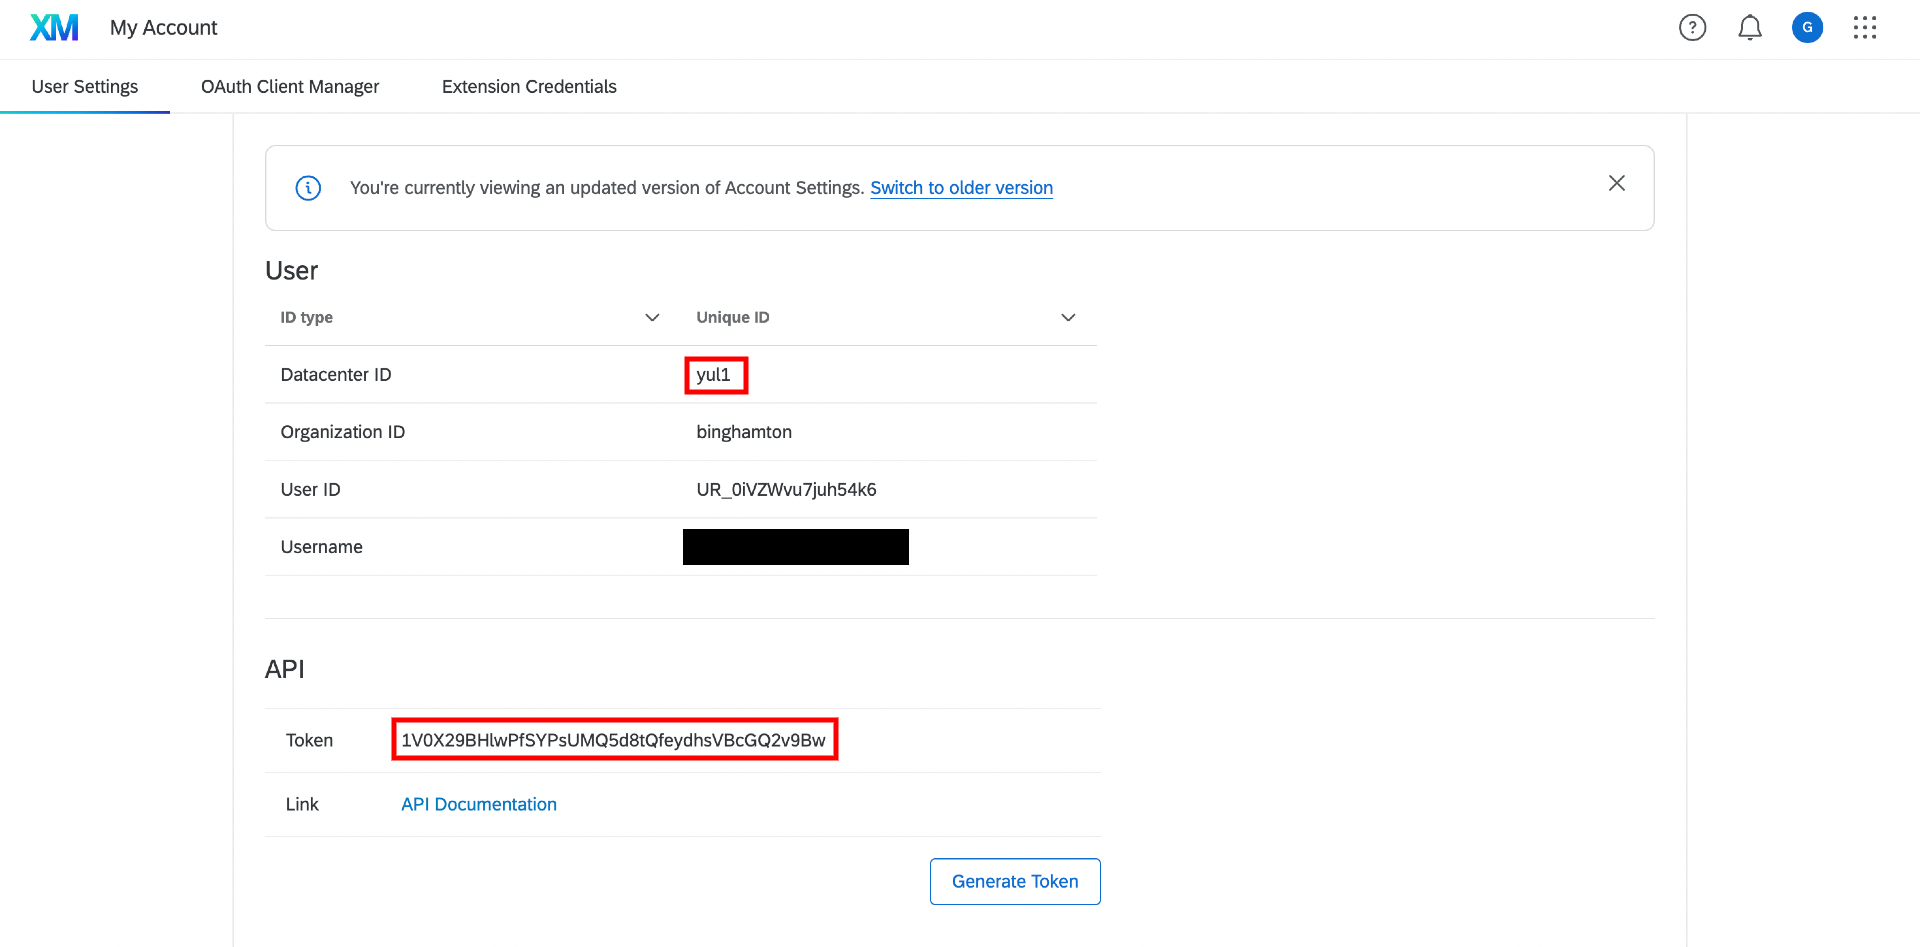
\includegraphics[keepaspectratio]{images/qualtrics_info_ex.png}}

}

\caption{Qualtrics Info}

\end{figure}%

When you log into Qualtrics, you're going to need to retrieve a few
pieces of data specific to your account and the survey that you want to
get live data from. Here, we've clicked our user icon in the top right
and gone to ``Account Settings.'' You're going to need these strings
later.

Next, you're going to need your survey ID. When you click on the survey
that you're getting live data from, the URL will look something like
this:
https://binghamton.yul1.qualtrics.com/survey-builder/SV\_6mOC1SaJbecAuP0/edit
The survey ID is the string between survey-builder/ and /edit, in this
case, being ``SV\_6mOC1SaJbecAuP0''

Getting into the actual code, we have the following steps: \#\# Import
necessary packages:

\begin{Shaded}
\begin{Highlighting}[]
\FunctionTok{library}\NormalTok{(httr)}
\FunctionTok{library}\NormalTok{(jsonlite)}
\FunctionTok{library}\NormalTok{(readr)}
\end{Highlighting}
\end{Shaded}

\section{Save important info to
variables:}\label{save-important-info-to-variables}

\begin{Shaded}
\begin{Highlighting}[]
\NormalTok{api\_token }\OtherTok{\textless{}{-}} \StringTok{"1V0X29BHlwPfSYPsUMQ5d8tQfeydhsVBcGQ2v9Bw"}
\NormalTok{data\_center }\OtherTok{\textless{}{-}} \StringTok{"yul1"}
\NormalTok{survey\_id }\OtherTok{\textless{}{-}} \StringTok{"SV\_6mOC1SaJbecAuP0"}

\NormalTok{base\_url }\OtherTok{\textless{}{-}} \FunctionTok{paste0}\NormalTok{(}\StringTok{"https://"}\NormalTok{, data\_center, }\StringTok{".qualtrics.com/API/v3"}\NormalTok{)}
\NormalTok{headers }\OtherTok{\textless{}{-}} \FunctionTok{add\_headers}\NormalTok{(}
  \StringTok{"X{-}API{-}TOKEN"} \OtherTok{=}\NormalTok{ api\_token,}
  \StringTok{"Content{-}Type"} \OtherTok{=} \StringTok{"application/json"}
\NormalTok{)}
\end{Highlighting}
\end{Shaded}

In this chunk, after saving our API key and survey ID info, we construct
the URL that we are going to scrape using the paste0 function (which
just combines the arguments into a single string with no spaces between
them). We add these specific headers because they are necessary
arguments for the API call.

\section{Start the export job}\label{start-the-export-job}

\begin{Shaded}
\begin{Highlighting}[]
\NormalTok{start\_response\_export }\OtherTok{\textless{}{-}} \ControlFlowTok{function}\NormalTok{(survey\_id) \{}
\NormalTok{  url }\OtherTok{\textless{}{-}} \FunctionTok{paste0}\NormalTok{(base\_url, }\StringTok{"/surveys/"}\NormalTok{, survey\_id, }\StringTok{"/export{-}responses"}\NormalTok{)}
\NormalTok{  body }\OtherTok{\textless{}{-}} \FunctionTok{list}\NormalTok{(}\AttributeTok{format =} \StringTok{"csv"}\NormalTok{)  }\CommentTok{\# Use CSV format here}
\NormalTok{  res }\OtherTok{\textless{}{-}} \FunctionTok{POST}\NormalTok{(url, headers, }\AttributeTok{body =} \FunctionTok{toJSON}\NormalTok{(body, }\AttributeTok{auto\_unbox =} \ConstantTok{TRUE}\NormalTok{))}
  \FunctionTok{stop\_for\_status}\NormalTok{(res)}
  \FunctionTok{content}\NormalTok{(res, }\AttributeTok{as =} \StringTok{"parsed"}\NormalTok{, }\AttributeTok{simplifyVector =} \ConstantTok{TRUE}\NormalTok{)}
\NormalTok{\}}
\end{Highlighting}
\end{Shaded}

This chunk creates the API endpoint and allows us to begin exporting. It
also gives us a progress report on how close the data is to being
exported!

\section{Poll for export completion}\label{poll-for-export-completion}

\begin{Shaded}
\begin{Highlighting}[]
\NormalTok{check\_export\_progress }\OtherTok{\textless{}{-}} \ControlFlowTok{function}\NormalTok{(progress\_id) \{}
\NormalTok{  url }\OtherTok{\textless{}{-}} \FunctionTok{paste0}\NormalTok{(base\_url, }\StringTok{"/surveys/"}\NormalTok{, survey\_id, }\StringTok{"/export{-}responses/"}\NormalTok{, progress\_id)}
  \ControlFlowTok{repeat}\NormalTok{ \{}
\NormalTok{    res }\OtherTok{\textless{}{-}} \FunctionTok{GET}\NormalTok{(url, headers)}
    \FunctionTok{stop\_for\_status}\NormalTok{(res)}
\NormalTok{    progress }\OtherTok{\textless{}{-}} \FunctionTok{content}\NormalTok{(res, }\AttributeTok{as =} \StringTok{"parsed"}\NormalTok{, }\AttributeTok{simplifyVector =} \ConstantTok{TRUE}\NormalTok{)}
    \ControlFlowTok{if}\NormalTok{ (progress}\SpecialCharTok{$}\NormalTok{result}\SpecialCharTok{$}\NormalTok{status }\SpecialCharTok{==} \StringTok{"complete"}\NormalTok{) \{}
      \FunctionTok{return}\NormalTok{(progress}\SpecialCharTok{$}\NormalTok{result}\SpecialCharTok{$}\NormalTok{fileId)}
\NormalTok{    \} }\ControlFlowTok{else} \ControlFlowTok{if}\NormalTok{ (progress}\SpecialCharTok{$}\NormalTok{result}\SpecialCharTok{$}\NormalTok{status }\SpecialCharTok{==} \StringTok{"failed"}\NormalTok{) \{}
      \FunctionTok{stop}\NormalTok{(}\StringTok{"Export failed"}\NormalTok{)}
\NormalTok{    \}}
    \FunctionTok{Sys.sleep}\NormalTok{(}\DecValTok{2}\NormalTok{)}
\NormalTok{  \}}
\NormalTok{\}}
\end{Highlighting}
\end{Shaded}

Once the export is ready, this chunk returns the ID for the file that we
can now download from the API.

\section{Download and read CSV file}\label{download-and-read-csv-file}

\begin{Shaded}
\begin{Highlighting}[]
\NormalTok{daily\_download\_responses\_csv }\OtherTok{\textless{}{-}} \ControlFlowTok{function}\NormalTok{(file\_id) \{}
\NormalTok{  url }\OtherTok{\textless{}{-}} \FunctionTok{paste0}\NormalTok{(base\_url, }\StringTok{"/surveys/"}\NormalTok{, survey\_id, }\StringTok{"/export{-}responses/"}\NormalTok{, file\_id, }\StringTok{"/file"}\NormalTok{)}
\NormalTok{  res }\OtherTok{\textless{}{-}} \FunctionTok{GET}\NormalTok{(url, headers)}
  \FunctionTok{stop\_for\_status}\NormalTok{(res)}
\NormalTok{  tmp }\OtherTok{\textless{}{-}} \FunctionTok{tempfile}\NormalTok{(}\AttributeTok{fileext =} \StringTok{".zip"}\NormalTok{)}
  \FunctionTok{writeBin}\NormalTok{(}\FunctionTok{content}\NormalTok{(res, }\StringTok{"raw"}\NormalTok{), tmp)}
\NormalTok{  unzip\_dir }\OtherTok{\textless{}{-}} \FunctionTok{tempdir}\NormalTok{()}
  \FunctionTok{unzip}\NormalTok{(tmp, }\AttributeTok{exdir =}\NormalTok{ unzip\_dir)}
\NormalTok{  csv\_file }\OtherTok{\textless{}{-}} \FunctionTok{list.files}\NormalTok{(unzip\_dir, }\AttributeTok{pattern =} \StringTok{"*.csv"}\NormalTok{, }\AttributeTok{full.names =} \ConstantTok{TRUE}\NormalTok{)}
  \FunctionTok{read\_csv}\NormalTok{(csv\_file)}
\NormalTok{\}}
\end{Highlighting}
\end{Shaded}

This chunk unpacks the output into a .csv file which makes it ready for
analysis!

\section{Main execution}\label{main-execution}

\begin{Shaded}
\begin{Highlighting}[]
\NormalTok{export\_response }\OtherTok{\textless{}{-}} \FunctionTok{start\_response\_export}\NormalTok{(survey\_id)}
\NormalTok{progress\_id }\OtherTok{\textless{}{-}}\NormalTok{ export\_response}\SpecialCharTok{$}\NormalTok{result}\SpecialCharTok{$}\NormalTok{progressId}
\NormalTok{file\_id }\OtherTok{\textless{}{-}} \FunctionTok{check\_export\_progress}\NormalTok{(progress\_id)}
\NormalTok{responses\_df }\OtherTok{\textless{}{-}} \FunctionTok{daily\_download\_responses\_csv}\NormalTok{(file\_id)}
\end{Highlighting}
\end{Shaded}

Finally, we set up our dataframes. These dataframes are now in your
environment and can update charts or tables every time you reload the
export!

\part{Tidy Data}

\chapter{Tidying your data with
tidyr}\label{tidying-your-data-with-tidyr}

\begin{tcolorbox}[enhanced jigsaw, title=\textcolor{quarto-callout-tip-color}{\faLightbulb}\hspace{0.5em}{📖 Learning Resources}, opacityback=0, colframe=quarto-callout-tip-color-frame, rightrule=.15mm, left=2mm, toprule=.15mm, leftrule=.75mm, titlerule=0mm, bottomtitle=1mm, breakable, arc=.35mm, toptitle=1mm, bottomrule=.15mm, coltitle=black, opacitybacktitle=0.6, colback=white, colbacktitle=quarto-callout-tip-color!10!white]

\begin{itemize}
\tightlist
\item
  \textbf{R for Data Science}:
  \href{https://r4ds.hadley.nz/data-tidy.html}{Data Tidying}
\item
  \textbf{Datacamp Course}:
  \href{https://www.datacamp.com/courses/reshaping-data-with-tidyr}{dplyr}
\item
  \textbf{Cheat Sheet}:
  \href{https://rstudio.github.io/cheatsheets/tidyr.pdf}{dplyr}
\item
  \textbf{Posit Interactive Page}:
  \href{https://rstudio.github.io/cheatsheets/html/tidyr.html}{dplyr}
\end{itemize}

\end{tcolorbox}

More coming soon!

\part{Report Transparently:}

\chapter{How to Read Me}\label{how-to-read-me}

This chapter introduces students to the basics of a read me file.

\hfill\break

\chapter{Read Me}\label{read-me}

A \texttt{readme.qmd} file instructs someone else to \emph{read me}. It
provides basic information and contextual information to a colleague who
wants to replicate or check your work.

To see an example of an excellent read me file, see ``zero sum report
read me file'':
\url{https://fripublichealth.quarto.pub/zerosum/readme-preview.html}

\chapter{How to Write Functions}\label{how-to-write-functions}

From Text to Code

This chapter introduces reproducible research practices by demonstrating
how to embed R code directly into manuscript text using Quarto. Students
learn to replace manually typed numbers with dynamic inline R code that
automatically updates when data changes, reducing errors and improving
research reproducibility. Through practical examples using survey data,
the chapter covers reporting sample sizes, calculating percentages,
formatting numbers as words, interpreting descriptive statistics tables,
and presenting statistical test results. By the end of this chapter,
students will be able to transform static numbers in their research
papers into dynamic, code-generated values that maintain accuracy
throughout the research process.

\hfill\break

\section{Purpose}\label{purpose-1}

In reproducible research, writing \emph{numbers} \emph{manually} (e.g.,
``We surveyed 120 people.'') can lead to errors if you import data later
(after you have collected 140 people). Instead, use \textbf{R functions}
inside \textbf{Quarto} to turn your results directly into sentences!

\section{First Setup the library:}\label{first-setup-the-library-1}

\begin{Shaded}
\begin{Highlighting}[]
\FunctionTok{library}\NormalTok{(tidyverse)}
\FunctionTok{library}\NormalTok{(psych)}
\FunctionTok{library}\NormalTok{(knitr)}
\FunctionTok{library}\NormalTok{(tibble)}
\FunctionTok{library}\NormalTok{(dplyr)}
\FunctionTok{library}\NormalTok{(tidyr)}
\FunctionTok{library}\NormalTok{(scales)     }\CommentTok{\# for number formatting like comma()}
\FunctionTok{library}\NormalTok{(english)    }\CommentTok{\# to convert numbers to words}
\FunctionTok{library}\NormalTok{(stringr)    }\CommentTok{\# for text functions like str\_c()}
\end{Highlighting}
\end{Shaded}

\section{Dataset: Example Survey
Data}\label{dataset-example-survey-data}

The dataset was collected on March 15, 2025 in the ANTH206 course:
\texttt{03152025ProlificHealthBeliefs.csv}.

\begin{Shaded}
\begin{Highlighting}[]
\CommentTok{\# Load your data}
\DocumentationTok{\#\#  "data/" is a folder called "data" where the dataset file is located}
\DocumentationTok{\#\# if your data is not in a folder, you can delete "data/"}
\NormalTok{select\_data }\OtherTok{\textless{}{-}} \FunctionTok{read.csv}\NormalTok{(}\StringTok{"data/03.15.2025.ProlificHealthBeliefs.csv"}\NormalTok{)}

\CommentTok{\# displays structures of R objects}
\FunctionTok{str}\NormalTok{(select\_data)}
\end{Highlighting}
\end{Shaded}

\section{Example 1: Reporting Sample Size in a Manuscript (using inline
R)}\label{example-1-reporting-sample-size-in-a-manuscript-using-inline-r}

\begin{Shaded}
\begin{Highlighting}[]
\NormalTok{\#| autorun: false}
\NormalTok{\#| completion: true}

\NormalTok{\# Example: find out total survey responses (\# of rows of data)}
\NormalTok{total\_responses \textless{}{-} nrow(select\_data)}

\NormalTok{\# print out total responses}
\NormalTok{total\_responses}
\end{Highlighting}
\end{Shaded}

\section{In your manuscript, write like
this:}\label{in-your-manuscript-write-like-this}

\begin{Shaded}
\begin{Highlighting}[]
\NormalTok{We surveyed a total of }\InformationTok{\textasciigrave{}r total\_responses\textasciigrave{}}\NormalTok{ participants.}
\end{Highlighting}
\end{Shaded}

When you render the output, you'll get:

\begin{Shaded}
\begin{Highlighting}[]
\NormalTok{We surveyed a total of 122 participants.}
\end{Highlighting}
\end{Shaded}

\section{Example 2: Report Numbers and
Percentages}\label{example-2-report-numbers-and-percentages}

You can combine counts and percentages easily.

\begin{Shaded}
\begin{Highlighting}[]
\NormalTok{\#| autorun: false}
\NormalTok{\#| completion: true}

\NormalTok{\# find out each total racial groups responses}
\NormalTok{asian\_responses \textless{}{-} sum(select\_data$RACIALIDENTITY.4 == "Asian")}
\NormalTok{black\_responses \textless{}{-} sum(select\_data$RACIALIDENTITY.4 == "Black")}
\NormalTok{white\_responses \textless{}{-} sum(select\_data$RACIALIDENTITY.4 == "White")}
\NormalTok{mixed\_other\_responses \textless{}{-} sum(select\_data$RACIALIDENTITY.4 == "Mixed/Other")}

\NormalTok{\# get the percentage of each racial groups}
\NormalTok{asian \textless{}{-} asian\_responses / total\_responses}
\NormalTok{black \textless{}{-} black\_responses / total\_responses}
\NormalTok{white \textless{}{-} white\_responses / total\_responses}
\NormalTok{mixed\_other \textless{}{-} mixed\_other\_responses / total\_responses}

\NormalTok{\# print out responses}
\NormalTok{asian\_responses}
\NormalTok{black\_responses}
\NormalTok{white\_responses}
\NormalTok{mixed\_other\_responses}

\NormalTok{\# print out percentage}
\NormalTok{asian}
\NormalTok{black}
\NormalTok{white}
\NormalTok{mixed\_other}
\end{Highlighting}
\end{Shaded}

\section{In your manuscript, write like
this:}\label{in-your-manuscript-write-like-this-1}

\begin{Shaded}
\begin{Highlighting}[]
\NormalTok{Out of }\InformationTok{\textasciigrave{}r total\_responses\textasciigrave{}}\NormalTok{ participants, The final sample was roughly balanced in terms of }
\NormalTok{racial identity (White: }\InformationTok{\textasciigrave{}r percent(white, accuracy = 0.1)\textasciigrave{}}\NormalTok{, }
\NormalTok{                 Black: }\InformationTok{\textasciigrave{}r percent(black, accuracy = 0.1)\textasciigrave{}}\NormalTok{,}
\NormalTok{                 Asian: }\InformationTok{\textasciigrave{}r percent(asian, accuracy = 0.1)\textasciigrave{}}\NormalTok{, }
\NormalTok{                 Mixed/Other: }\InformationTok{\textasciigrave{}r percent(mixed\_other, accuracy = 0.1)\textasciigrave{}}\NormalTok{).}
\end{Highlighting}
\end{Shaded}

When you render the output, you'll get:

\begin{Shaded}
\begin{Highlighting}[]
\NormalTok{Out of 122 participants, The final sample was roughly balanced in terms of racial identity}
\NormalTok{(White: 40.2\%, Black: 23.0\%, Asian: 18.9\%, Mixed/Other: 18.0\%).}
\end{Highlighting}
\end{Shaded}

\section{Example 3: Capitalizing and Writing Numbers as
Words}\label{example-3-capitalizing-and-writing-numbers-as-words}

For more formal writing, report numbers as words:

\section{In your manuscript, write like
this:}\label{in-your-manuscript-write-like-this-2}

\begin{Shaded}
\begin{Highlighting}[]
\NormalTok{A total of }\InformationTok{\textasciigrave{}r str\_to\_title(as.character(english(total\_responses)))\textasciigrave{}}\NormalTok{ participants were included in the analysis.}
\end{Highlighting}
\end{Shaded}

When you render the output, you'll get:

\begin{Shaded}
\begin{Highlighting}[]
\NormalTok{A total of One Hundred And Twenty{-}Two participants were included in the analysis.}
\end{Highlighting}
\end{Shaded}

\section{Example 4: Interpret a table by using inline R code (Mean, SD,
Range)}\label{example-4-interpret-a-table-by-using-inline-r-code-mean-sd-range}

\begin{Shaded}
\begin{Highlighting}[]
\CommentTok{\# Define Continuous Variables}
\NormalTok{continuous\_vars }\OtherTok{\textless{}{-}} \FunctionTok{c}\NormalTok{(}
  \StringTok{"AGE"}\NormalTok{, }\StringTok{"SOCIALSTATUS"}\NormalTok{, }\StringTok{"POLITICALBELIEFS"}\NormalTok{,}
  \FunctionTok{paste0}\NormalTok{(}\StringTok{"ZEROSUM\_"}\NormalTok{, }\DecValTok{1}\SpecialCharTok{:}\DecValTok{11}\NormalTok{)}
\NormalTok{)}

\NormalTok{desc\_table\_continuous }\OtherTok{\textless{}{-}}\NormalTok{ select\_data }\SpecialCharTok{\%\textgreater{}\%}
  \FunctionTok{select}\NormalTok{(}\FunctionTok{all\_of}\NormalTok{(continuous\_vars)) }\SpecialCharTok{\%\textgreater{}\%}
\NormalTok{  psych}\SpecialCharTok{::}\FunctionTok{describe}\NormalTok{() }\SpecialCharTok{\%\textgreater{}\%}
\NormalTok{  tibble}\SpecialCharTok{::}\FunctionTok{rownames\_to\_column}\NormalTok{(}\AttributeTok{var =} \StringTok{"Variable"}\NormalTok{) }\SpecialCharTok{\%\textgreater{}\%}
  \FunctionTok{select}\NormalTok{(Variable, n, mean, median, sd, min, max)}

\CommentTok{\# Remove font specifications from nice\_table}
\NormalTok{knitr}\SpecialCharTok{::}\FunctionTok{kable}\NormalTok{(desc\_table\_continuous,}
             \AttributeTok{digits =} \DecValTok{2}\NormalTok{)}
\end{Highlighting}
\end{Shaded}

\begin{longtable}[]{@{}lrrrrrr@{}}
\caption{Descriptive Statistics Table for Continuous
Variables}\tabularnewline
\toprule\noalign{}
Variable & n & mean & median & sd & min & max \\
\midrule\noalign{}
\endfirsthead
\toprule\noalign{}
Variable & n & mean & median & sd & min & max \\
\midrule\noalign{}
\endhead
\bottomrule\noalign{}
\endlastfoot
AGE & 121 & 36.10 & 33.0 & 12.73 & 19 & 73 \\
SOCIALSTATUS & 122 & 5.30 & 5.5 & 1.78 & 1 & 9 \\
POLITICALBELIEFS & 120 & 3.67 & 4.0 & 1.35 & 1 & 6 \\
ZEROSUM\_1 & 122 & 3.92 & 4.0 & 1.78 & 1 & 7 \\
ZEROSUM\_2 & 121 & 4.75 & 5.0 & 1.59 & 1 & 7 \\
ZEROSUM\_3 & 121 & 4.92 & 5.0 & 1.49 & 1 & 7 \\
ZEROSUM\_4 & 121 & 3.07 & 3.0 & 1.69 & 1 & 7 \\
ZEROSUM\_5 & 122 & 2.84 & 3.0 & 1.75 & 1 & 7 \\
ZEROSUM\_6 & 121 & 3.43 & 3.0 & 2.07 & 1 & 7 \\
ZEROSUM\_7 & 120 & 3.52 & 4.0 & 1.81 & 1 & 7 \\
ZEROSUM\_8 & 121 & 2.93 & 3.0 & 1.63 & 1 & 7 \\
ZEROSUM\_9 & 121 & 2.59 & 2.0 & 1.74 & 1 & 7 \\
ZEROSUM\_10 & 122 & 3.20 & 3.0 & 1.75 & 1 & 7 \\
ZEROSUM\_11 & 121 & 3.17 & 3.0 & 1.74 & 1 & 7 \\
\end{longtable}

\section{In your manuscript, write like
this:}\label{in-your-manuscript-write-like-this-3}

\begin{Shaded}
\begin{Highlighting}[]
\NormalTok{Descriptive statistics for all study variables are presented in Continuous Descriptive Statistics Table. }
\NormalTok{The sample consisted of }\InformationTok{\textasciigrave{}r nrow(select\_data)\textasciigrave{}}\NormalTok{ participants, }
\NormalTok{with a mean age of }\InformationTok{\textasciigrave{}r round(desc\_table\_continuous$mean[desc\_table\_continuous$Variable == "AGE"], 2)\textasciigrave{}} 
\NormalTok{years (SD = }\InformationTok{\textasciigrave{}r round(desc\_table\_continuous$sd[desc\_table\_continuous$Variable == "AGE"], 2)\textasciigrave{}}\NormalTok{, }
\NormalTok{range = }\InformationTok{\textasciigrave{}r desc\_table\_continuous$min[desc\_table\_continuous$Variable == "AGE"]\textasciigrave{}}
\NormalTok{– }\InformationTok{\textasciigrave{}r desc\_table\_continuous$max[desc\_table\_continuous$Variable == "AGE"]\textasciigrave{}}\NormalTok{). }

\NormalTok{Participants reported a mean social status of }
\InformationTok{\textasciigrave{}r round(desc\_table\_continuous$mean[desc\_table\_continuous$Variable == "SOCIALSTATUS"], 2)\textasciigrave{}} 
\NormalTok{(SD = }\InformationTok{\textasciigrave{}r round(desc\_table\_continuous$sd[desc\_table\_continuous$Variable == "SOCIALSTATUS"], 2)\textasciigrave{}}\NormalTok{) on a 10{-}point scale.}
\end{Highlighting}
\end{Shaded}

When you render the output, you'll get:

\begin{Shaded}
\begin{Highlighting}[]
\NormalTok{Descriptive statistics for all study variables are presented in Continuous Descriptive Statistics Table. }
\NormalTok{The sample consisted of 122 participants, with a mean age of 36.1 years (SD = 12.73, range = 19 – 73). }
\NormalTok{Participants reported a mean social status of 5.3 (SD = 1.78) on a 10{-}point scale.}
\end{Highlighting}
\end{Shaded}

\section{Example 5: Interpret P-value in a Kruskal-Wallis Test by using
inline R
code}\label{example-5-interpret-p-value-in-a-kruskal-wallis-test-by-using-inline-r-code}

\begin{Shaded}
\begin{Highlighting}[]
\NormalTok{\#| label: Kruskal{-}Wallis zerosum1}

\NormalTok{kw.ZEROSUM\_1.party \textless{}{-} kruskal.test(ZEROSUM\_1 \textasciitilde{} POLITICALPARTY, data = select\_data)}
\NormalTok{kw.ZEROSUM\_1.party}
\end{Highlighting}
\end{Shaded}

\section{In your manuscript, write like
this:}\label{in-your-manuscript-write-like-this-4}

\begin{Shaded}
\begin{Highlighting}[]
\NormalTok{There was no significant difference in ZEROSUM\_1 scores across political party groups, }
\NormalTok{Kruskal{-}Wallis χ²(}\InformationTok{\textasciigrave{}r kw.ZEROSUM\_1.party$parameter\textasciigrave{}}\NormalTok{) = }\InformationTok{\textasciigrave{}r round(kw.ZEROSUM\_1.party$statistic, 2)\textasciigrave{}}\NormalTok{, }
\NormalTok{*p* = }\InformationTok{\textasciigrave{}r signif(kw.ZEROSUM\_1.party$p.value, 3)\textasciigrave{}}\NormalTok{.}
\end{Highlighting}
\end{Shaded}

When you render the output, you'll get:

\begin{Shaded}
\begin{Highlighting}[]
\NormalTok{There was no significant difference in ZEROSUM\_1 scores across political party groups, }
\NormalTok{Kruskal{-}Wallis χ²(2) = 1.5, p = 0.473.}
\end{Highlighting}
\end{Shaded}





\end{document}
